% Uncomment this to make slides with overlays:
%\documentclass[slides]{beamer}

% Uncomment these (but comment the above \documentclass line) to make handouts:
\documentclass[handout]{beamer}

% Uncomment these to have more than one slide per page
\usepackage{pgfpages}
\pgfpagesuselayout{2 on 1}[border shrink=5mm]
\pgfpageslogicalpageoptions{1}{border code=\pgfusepath{stroke}}
\pgfpageslogicalpageoptions{2}{border code=\pgfusepath{stroke}}

\usepackage[]{graphicx, color, hyperref}

\mode<presentation>
{
	%\usetheme[secheader]{Boadilla}
	%\usecolortheme[rgb={.835, .102,.169}]{structure}  
	\usetheme[width= 0cm]{Goettingen}
	%\setbeamercovered{transparent}
}
\setbeamertemplate{navigation symbols}{}
\setbeamertemplate{footline}[frame number]

\definecolor{blue2}{rgb}{0.278,0.278,0.729} 
\newcommand{\blue}[1]{\textcolor{blue2}{#1}}
\newcommand{\white}[1]{\textcolor{white}{#1}}
\newcommand{\red}[1]{\textcolor{red}{#1}}
\newcommand{\xbar}{\overline{x}}
\newcommand{\ybar}{\overline{y}}
\newcommand{\phat}{\widehat{p}}
\newcommand{\prob}{\mbox{Pr}}
\newcommand{\E}{\mathbb{E}}
\newcommand{\Var}{\mbox{Var}}
\newcommand{\cp}{\oplus}
\newcommand{\cm}{\circleddash}

\title{Lecture 14: Hypothesis Testing}
\author{Chapter 4.3}
\date{}


\begin{document}
%------------------------------------------------------------------------------
\begin{frame}
\titlepage
\end{frame}
%------------------------------------------------------------------------------


%-------------------------------------------------------------------------------
\begin{frame}
\frametitle{Previously: Confidence Intervals}
If we know the sampling distribution of $\xbar$ is Normal with
\begin{itemize}
\item mean equal to the true unknown population mean $\mu$
\item standard error $SE = \frac{s}{\sqrt{n}}$
\end{itemize}
then we can use the Normal model build confidence intervals.

\pause\vspace{0.5cm}

i.e.
\[
\left[\xbar - z^* SE, \mbox{  }\xbar + z^* SE\right] = 
\left[\xbar - z^* \frac{s}{\sqrt{n}}, \mbox{  }\xbar + z^* \frac{s}{\sqrt{n}}\right]
\]
i.e. where $z^*$ is the value from the normal table that sets the confidence level.  Ex:  $z^*=1.96$ sets a 95\% confidence interval.  

\end{frame}
%-------------------------------------------------------------------------------



%-------------------------------------------------------------------------------
\begin{frame}
\frametitle{Previously: How to Interpret a Confidence Interval}

\begin{center}
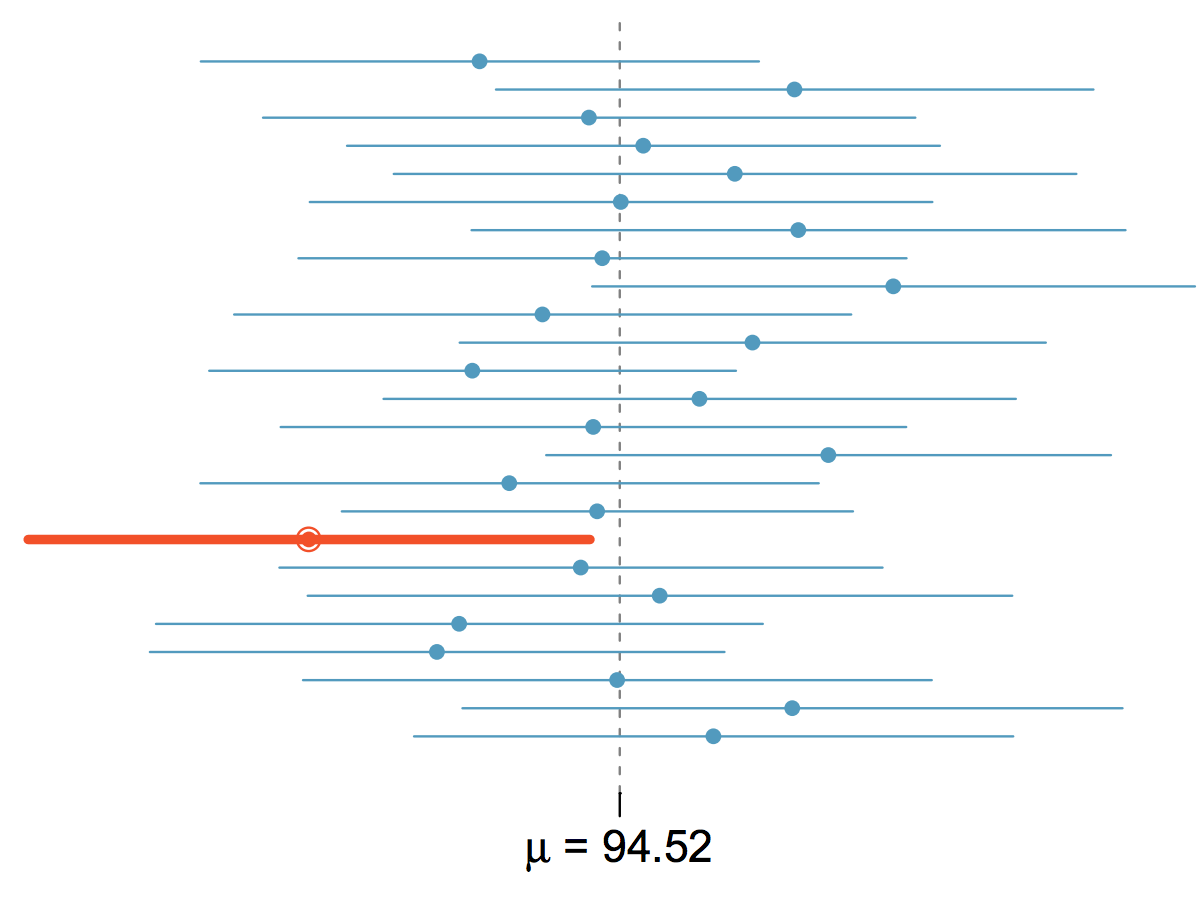
\includegraphics[width=8cm]{figure/CI.png}
\end{center}

\end{frame}
%-------------------------------------------------------------------------------



%------------------------------------------------------------------------------
\begin{frame}[fragile]
\frametitle{Goals for Today}

\begin{itemize}
\item Introduce Hypothesis Testing Framework
\item Testing Hypotheses Using Confidence Intervals
\item Types of Errors
\item Testing Hypotheses Using p-Values
\end{itemize}

\end{frame}
%------------------------------------------------------------------------------



%-------------------------------------------------------------------------------
\begin{frame}
\frametitle{Statistical Hypothesis Testing}
(For now) A \blue{hypothesis} is a claim about a population parameter.

\vskip 0.25cm

\pause A \blue{hypothesis test} is a method for using sample data to decide between two competing hypotheses about the population parameter:
\begin{itemize}
\pause \item A \blue{null hypothesis $H_0$}.\\
i.e. the \blue{status quo} that is initially assumed to be true, but will be tested. 
\pause \item An \blue{alternative hypothesis $H_A$}.\\
i.e. the \blue{challenger}.
\end{itemize}

\end{frame}
%-------------------------------------------------------------------------------



%-------------------------------------------------------------------------------
\begin{frame}
\frametitle{Examples}
\begin{itemize}
\item We flip a coin many times and start to suspect that it is biased:
\begin{itemize}
\pause \item $H_0$: the coin is fair.  i.e. the probability of heads is $p=0.5$
\item $H_A$: the coin is not fair.  i.e. $p \neq 0.5$
\end{itemize}
\pause \item From book:  The average 10 mile run time for the Cherry Blossom Run in 2006 $\mu_{2006}$ was 93.29 min.  Researchers suspect $\mu_{2012}$ was different:
\begin{itemize}
\pause \item $H_0$: the average time was the same. i.e. $\mu_{2012} = 93.29$
\item $H_A$: the average time was different. i.e. $\mu_{2012} \neq 93.29$
\end{itemize}
\end{itemize}
\end{frame}
%-------------------------------------------------------------------------------



%-------------------------------------------------------------------------------
\begin{frame}
\frametitle{Crucial Concept: Conclusions of Hypothesis Tests}
There are two potential outcomes of a hypothesis test.  Either we
\pause \begin{itemize}
\item reject $H_0$ in favor of $H_A$
\item fail to reject $H_0$
\end{itemize}

\vspace{0.5cm}

\pause Note the difference between \blue{accepting $H_0$} \& \blue{failing to reject $H_0$}
\begin{itemize}
\pause \item ``accepting $H_0$'' is saying we are sure $H_0$ is true
\pause \item ``failing to reject $H_0$'' is saying something not as strong:  \blue{we do not have enough evidence to reject $H_0$}.
\end{itemize}

\end{frame}
%-------------------------------------------------------------------------------



%-------------------------------------------------------------------------------
\begin{frame}
\frametitle{Analogy:  US Criminal Justice System}


In a recent trial, George Zimmerman was found \blue{not guilty} by the jury.  The jury's verdict does NOT make any statement about the defendant being \blue{innocent}, rather that there was not enough evidence to prove beyond a reasonable doubt that they were guilty.

\end{frame}
%-------------------------------------------------------------------------------



%-------------------------------------------------------------------------------
\begin{frame}
\frametitle{Analogy:  US Criminal Justice System}

Let's compare criminal trials to hypothesis tests:

\vspace{0.5cm}

\pause \blue{Truth}:
\begin{itemize}
\pause \item Truth about the defendant: innocence vs guilt
\pause \item Truth about the hypothesis: $H_0$ or $H_A$
\end{itemize}

\vspace{0.25cm}

\pause \blue{Decision}:
\begin{itemize}
\pause \item Verdict:  not guilty vs guilty
\pause \item Test outcome: ``Do not reject $H_0$'' vs ``Reject $H_0$''
\end{itemize}

\end{frame}
%-------------------------------------------------------------------------------



%-------------------------------------------------------------------------------
\begin{frame}
\frametitle{Testing Hypotheses Using Confidence Intervals}

Back to example:  The average race time $\mu_{2006}$ for 2006 was 93.29 min.  Researchers suspect $\mu_{2012}$ was different:
\begin{itemize}
\pause \item $H_0$: the average time was the same. i.e. $\mu_{2012} = 93.29$
\pause \item $H_A$: the average time was different. i.e. $\mu_{2012} \neq 93.29$
\end{itemize}

\pause \vspace{0.5cm}

93.29 is called the \blue{null value $\mu_{0}$} (mu-naught) since it represents the value of the parameter if the null hypothesis is true.

\pause \vspace{0.5cm}

They take a sample of size $n=100$ times from 2012 and find that $\xbar=95.61$ and $s=15.78$

\pause \vspace{0.5cm}

The average time $\xbar=95.61$, our estimate of $\mu_{2012}$, is greater than 93.29.  Is that enough to say that the times are different?

\end{frame}
%-------------------------------------------------------------------------------



%-------------------------------------------------------------------------------
\begin{frame}
\frametitle{Testing Hypotheses Using Confidence Intervals}

Recall that a 95\% confidence interval for the population mean $\mu$ based on a sample of points $x_1, \ldots, x_n$ is 

\begin{eqnarray*}
\pause \left[\overline{x} - 1.96 \times\frac{s}{\sqrt n}\right.,
\left.\overline{x} + 1.96 \times\frac{s}{\sqrt n}\right]
\pause = \left[92.45\right., \left.98.77\right]
\end{eqnarray*}


\end{frame}
%-------------------------------------------------------------------------------



%-------------------------------------------------------------------------------
\begin{frame}
\frametitle{Testing Hypotheses Using Confidence Intervals}

Since the 2006 \blue{null value} 93.29 falls in the range of plausible values, we cannot say the null hypothesis is implausible.  i.e. we fail to reject the null hypothesis that the 2006 and 2012 times are the same.  

\pause \vspace{0.25cm}

Again, we are NOT saying that the 2006 and 2012 times are the same.  Just that there is insufficient evidence to suggest otherwise.


\end{frame}
%-------------------------------------------------------------------------------



%-------------------------------------------------------------------------------
\begin{frame}
\frametitle{Decision Errors}
Hypothesis tests will get things right sometimes and wrong sometimes:
\pause \begin{center}
  \begin{tabular}{cc|cc}
     \multicolumn{2}{c}{}  & \multicolumn{2}{c}{\textbf{Test conclusion}} \\ 
     &  & do not reject $H_0$ & reject $H_0$ in favor of $H_A$ \\ 
\hline
    \textbf{Truth} & $H_0$ true & OK & \blue{Type I Error} \\ 
     & $H_A$ true & \blue{Type II Error} & OK \\ 
    \hline
  \end{tabular}
\end{center}

\vspace{0.25cm}

\pause Two kinds of errors:
\begin{itemize}
\pause \item \blue{Type I Error}: a false positive
\pause \item \blue{Type II Error}: a false negative
\end{itemize}

\end{frame}
%-------------------------------------------------------------------------------



%-------------------------------------------------------------------------------
\begin{frame}
\frametitle{Decision Errors}
\begin{itemize}
\item There is a trade-off between these two error rates: procedures with lower type I error rates typically have higher type II error rates and vice versa
\pause \item In other words, there is almost never a perfect test that makes no type I errors while making no type II errors
\pause \item Some sort of balance between the two is required
\end{itemize}
\end{frame}
%-------------------------------------------------------------------------------



%-------------------------------------------------------------------------------
\begin{frame}
\frametitle{Example:  US Criminal Justice System}
Defendants must be proven ``guilty beyond a reasonable doubt''  i.e. \blue{in theory} they would rather let a guilty person go free, than put an innocent person in jail.

\vskip 0.25cm
\pause So let:
\begin{itemize}
\item $H_0$: the defendant is innocent
\item $H_A$: the defendant is guilty
\end{itemize}
\pause thus rejecting $H_0$ corresponds to a guilty verdict.  i.e. putting them in jail
\vskip 0.25cm
\pause In this case:
\begin{itemize}
\item A type I error is putting an innocent person in jail\\
(considered worse)
\item A type II error is letting a guilty person go free.  
\end{itemize}
\end{frame}
%-------------------------------------------------------------------------------



%-------------------------------------------------------------------------------
\begin{frame}
\frametitle{Example:  Airport Screening}
An example of where type II error is much more serious:  \blue{airport screening}.  

\vskip 0.25cm
\pause Let:
\begin{eqnarray*}
H_0: && \mbox{passenger X does not have a bomb/weapon}\\
H_A: && \mbox{passenger X has a bomb/weapon}
\end{eqnarray*}
\pause Failing to reject $H_0$ when $H_0$ is false corresponds to not ``patting down'' passenger X when they really have a bomb/weapon.  This is disastrous!
\vskip 0.25cm
\pause Hence the long lines at airport security.  
\end{frame}
%-------------------------------------------------------------------------------



%-------------------------------------------------------------------------------
\begin{frame}
\frametitle{Significance Level}
Hypothesis testing is built around rejecting or failing to reject the null hypothesis\\
i.e. we do not reject $H_0$ unless we have \blue{strong evidence}.

\pause \vspace{0.5cm}

As a general rule of thumb, for those cases when $H_0$ is true, we do not want to incorrectly reject $H_0$ more than 5\% of the time.  In this case $\alpha = 0.05 = 5\%$ is the \blue{significance level}.  

\pause \vspace{0.5cm}

Using the procedure to create 95\% confidence intervals earlier, we expect it to miss the true population parameter 5\% of the time.  This corresponds to $\alpha=0.05$.   
\end{frame}
%-------------------------------------------------------------------------------



%-------------------------------------------------------------------------------
\begin{frame}
\frametitle{p-Values}
Thought experiment:  Say you flip a coin you think is fair 1000 times.  Thus you expect 500 heads.   Now say you observe
\begin{itemize}
\pause \item 501 heads? Do you think the coin is biased?
\pause \item 525 heads? Do you think the coin is biased?
\pause \item 900 heads? Do you think the coin is biased?
\end{itemize}
\pause Intuitively, a \blue{p-value} quantifies how \blue{extreme} an observation is given the null hypothesis.  
\vskip 0.25cm
\pause The smaller the p-value, the more \blue{extreme} the observation, where the meaning of extreme depends on the context.  
\end{frame}
%-------------------------------------------------------------------------------



%-------------------------------------------------------------------------------
\begin{frame}
\frametitle{p-Value Definition}
The \blue{p-value} or \blue{observed significance level} is the probability of observing a test statistic as extreme or more extreme (in favor of the alternative) as the one observed, assuming $H_0$ is true.

\vspace{0.5cm}

\pause It is \blue{NOT} the probability of $H_0$ being true.  This is the most common misinterpretation of the $p$-value.

\end{frame}
%-------------------------------------------------------------------------------



%-------------------------------------------------------------------------------
\begin{frame}
\frametitle{Example:  Exercise 4.28 on Page 177 on Sleep}
A poll found that college students sleep about 7 hours a night.  Researchers suspect that Reedies sleep more.  They use a sample of $n=110$ Reedies to investigate this claim at an $\alpha=0.05$ level.  

\vspace{0.5cm}

\pause Let $\mu$ be the true \# of hours Reedies sleep a night:

\pause \begin{itemize}
\item $H_0: \mu = \mu_0 = 7$
\item $H_A: \mu > 7$
\end{itemize}

\end{frame}
%-------------------------------------------------------------------------------



%-------------------------------------------------------------------------------
\begin{frame}
\frametitle{Example:  Exercise 4.28 on Page 177 on Sleep}
Researchers find that $\xbar = 7.42$ and $s=1.75$.  Before we proceed, we check the 3 conditions
\begin{enumerate}
\pause \item Independence: the sample size $n=110$ is less than 10\% of 1,453 (Reed enrollment)
\pause \item The sample size is greater than $30$
\pause \item The distribution of the $n=110$ observations (Figure 4.14) is not too skewed.
\end{enumerate}

\end{frame}
%-------------------------------------------------------------------------------



%-------------------------------------------------------------------------------
\begin{frame}
\frametitle{Example:  Exercise 4.28 on Page 177 on Sleep}

\blue{Question to keep in mind}:  What if the null hypothesis were true (i.e. the null value $\mu_0=7$)?

\pause \vspace{0.5cm}

How likely are we to observe $\xbar=7.42$ or something more extreme in favor of the alternative, i.e. greater?  Using the $z$-score of $\xbar$ and plots.  

\pause \vspace{0.5cm}

Remember in general
\[
z = \frac{x-\mu}{\sigma}
\]
\pause So in our case for $\xbar$
\[
z = \frac{\xbar - \mu \mbox{ when $H_0$ is true }}{SE} = \frac{\xbar - \mu_0}{SE} = \frac{7.42 - 7}{\frac{1.75}{\sqrt{110}}} = 2.47
\]


\end{frame}
%-------------------------------------------------------------------------------



%-------------------------------------------------------------------------------
\begin{frame}
\frametitle{Example:  Exercise 4.28 on Page 177 on Sleep}

If the null hypothesis were true, then $\xbar$ would have come from the following nearly normal distribution.  The $p$-Value is 0.007 since:

\begin{center}
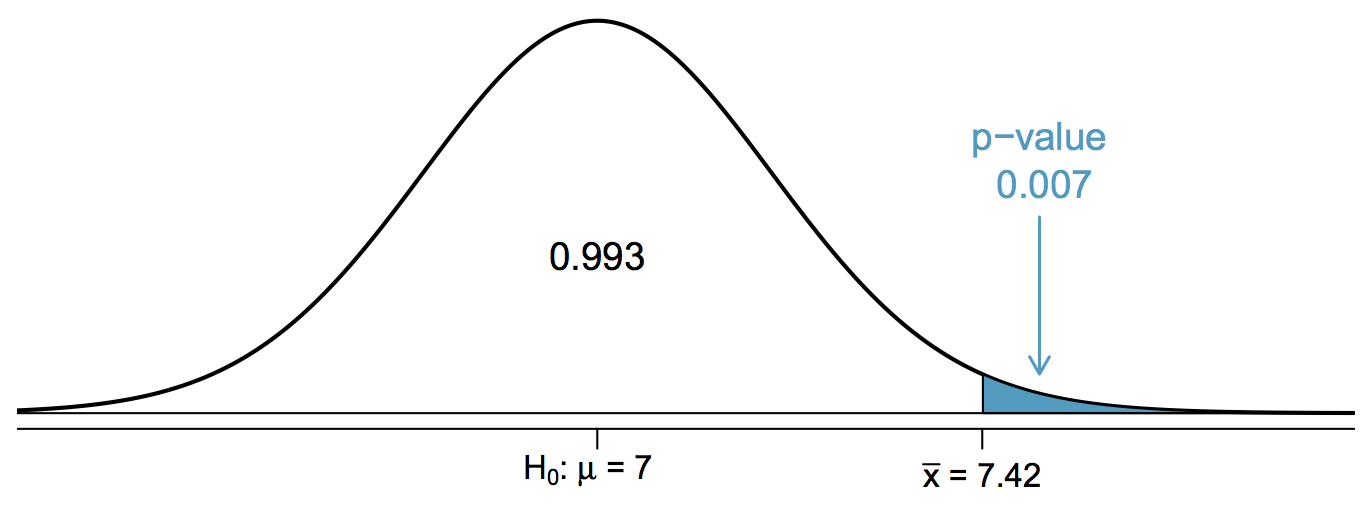
\includegraphics[width=\textwidth]{figure/pvalue.png}
\end{center}

\end{frame}
%-------------------------------------------------------------------------------



%-------------------------------------------------------------------------------
\begin{frame}
\frametitle{Example:  Exercise 4.28 on Page 177 on Sleep}

\blue{Correct interpretation}:  If the null hypothesis is true, the probability of observing a sample mean $\xbar=7.42$ or greater from a sample of size $n=110$ is only 0.007.  

\pause \vspace{0.5cm}
The p-value quantifies how strongly the data favor $H_A$ over $H_0$.  A small $p$-value corresponds to sufficient evidence to reject $H_0$ in favor of $H_A$.  


\pause \vspace{0.5cm}
Final decision.  Since we set $\alpha=0.05$ \blue{beforehand} and the p-value $0.007 < 0.05 = \alpha$, we reject the null hypothesis.  i.e. based on evidence, we believe Reedies sleep more than 7 hours a night.  

\end{frame}
%-------------------------------------------------------------------------------






















%------------------------------------------------------------------------------
\begin{frame}[fragile]
\frametitle{Next Time}

\begin{itemize}
\item More Hypothesis Testing
\item Central Limit Theorem
\end{itemize}


\end{frame}
%------------------------------------------------------------------------------







\end{document}




%-------------------------------------------------------------------------------
\begin{frame}
\frametitle{One vs Two Sided Hypothesis Tests}
This is a \blue{one-sided} hypothesis test.  Our test of a fair vs non fair coin was \blue{two-sided} since the alternative hypothesis was $H_A: p \neq 0.5$ i.e. $p>0.5$ or $p<0.5$
\end{frame}
%-------------------------------------------------------------------------------



%-------------------------------------------------------------------------------
\begin{frame}
\frametitle{Specifying a Test Procedure}
What is typically done is:
\begin{itemize}
\item Pick a desired $\alpha$ significance level and ``clamp'' the test to this $\alpha$.  Typical values include 0.10, 0.05, 0.01 and 0.001
\item Then pick the test that minimizes $\beta$.  
\end{itemize}
\vskip 0.25cm
So if you're in a situation where:
\begin{itemize}
\item Type I errors are much more serious than a type II error, set $\alpha$ to be lower and hence $\beta$ will be higher
\item Type II errors are much more serious, set $\beta$ to be lower and hence $\alpha$ will be higher
\end{itemize}
\end{frame}
%-------------------------------------------------------------------------------







